% TODAES journal format.  TODAES requires submissions to be prepared for
% double-anonymous review from 1 March 2026, so "anonymous" stays on and the
% author block below stays a placeholder.  For the camera-ready drop "review"
% (line numbers) and "anonymous" and paste in the real block, which is kept in
% paper/authors_cameraready.tex and gitignored so that it never reaches the
% anonymised review mirror; for a double-spaced reviewing copy swap "acmsmall"
% for "manuscript".
\documentclass[acmsmall,review,anonymous]{acmart}

% acmart already provides graphicx, booktabs, amsmath, amssymb, hyperref, url
% and xcolor; loading cite/hyperref again would clash with its natbib setup.
\usepackage{multirow}
\usepackage{algorithm}
\usepackage[noend]{algpseudocode}

% auto-generated by scripts/make_numbers.py -- do not edit
\newcommand{\AblationText}{No single removal is resolvable over 20 seeds per variant, every figure paired against the full system on shared seeds.  In order of damage: mutation guidance -2.4\% ($p=0.18$), candidate injection -1.8\% ($p=0.18$), space refinement -1.7\% ($p=0.35$), warm start -0.1\% ($p=1.00$), the proposal distribution alone +0.4\% ($p=1.00$); removing guidance altogether, NSGA-II, costs -1.6\%.  At this sample size, with a whole-system effect of a few percent, an ablation cannot apportion it between four overlapping operators, and these figures are not a ranking.  One split is worth reading, because the mutation-guidance row deletes two mechanisms at once.  Keeping the LLM local search and dropping only the proposal distribution costs \NoPriorGain\% ($p=\NoPriorP$) against \NoMutGain\% ($p=\NoMutP$) for dropping both; compared directly the two differ by \HalfSplit\% over \HalfSplitWins\ pairs ($p=\HalfSplitP$), the one comparison here that resolves, and it says the local search carries that operator while the proposal distribution does not.  Single removals also cost more than removing guidance entirely, so the operators interact.  The rest of the attribution comes from Section~\ref{sec:prior}, which varies one mechanism against a matched alternative instead of deleting it.}
\newcommand{\AppsText}{Quality degrades gracefully along the front, and design ALG-5 cuts the power--delay product from 66.6\,fJ to 23.4\,fJ, a 65\% reduction, while keeping LeNet-5 top-1 within one point of exact.  Read in pairs, the table repeats on the application side what Section~\ref{sec:sota16} showed on the circuit side: at matched \nmed{} the Approx-LG design matches the published design's image quality and stays within a point of its top-1 while spending 30 to 54\% less energy.  The most aggressive point is the exception: ALG-6 is 90\% cheaper than ALM\_SOA\_W12 at the same \nmed{}, but its relative error is 13$\times$ larger and the classifier collapses to 60.8\% where the logarithmic reference holds 98.2\%.  Relative error on small activations is exactly the axis a truncation-heavy design gives up, which is why the useful output of the search is the whole front, not one design.}
\newcommand{\BoxGainHi}{+3.3}
\newcommand{\BoxGainLo}{+0.4}
\newcommand{\BoxSig}{2}
\newcommand{\BreakEvenNSGA}{0.98}
\newcommand{\BreakEvenRF}{1.44}
\newcommand{\BreakEvenSham}{0.58}
\newcommand{\Budget}{400}
\newcommand{\DeadGap}{-1.1}
\newcommand{\DeadHV}{0.0716}
\newcommand{\DeadHVN}{0.0724}
\newcommand{\DeadP}{0.12}
\newcommand{\DeadRuns}{20}
\newcommand{\DeadWins}{6/20}
\newcommand{\DeadWorst}{-10}
\newcommand{\EffectA}{0.60}
\newcommand{\EpsGain}{-12.0}
\newcommand{\EpsP}{0.97}
\newcommand{\EpsWins}{18/30}
\newcommand{\EqTimeEvals}{1068}
\newcommand{\EqTimeNSGA}{-1.55}
\newcommand{\EqTimeNSGACI}{[-2.26,\,-0.80]}
\newcommand{\EqTimeNSGAP}{0.001}
\newcommand{\EqTimeRF}{-1.97}
\newcommand{\EqTimeRFCI}{[-2.60,\,-1.30]}
\newcommand{\EqTimeRFP}{$<$0.001}
\newcommand{\EqTimeSeconds}{356}
\newcommand{\EqTimeSham}{-0.84}
\newcommand{\EqTimeShamCI}{[-1.64,\,+0.03]}
\newcommand{\EqTimeShamP}{0.064}
\newcommand{\EvalsApproxLG}{338}
\newcommand{\EvalsSixteenS}{320}
\newcommand{\EvalsSixteenU}{384}
\newcommand{\ExpertSixteenS}{+1.5}
\newcommand{\ExpertSixteenSP}{0.021}
\newcommand{\ExpertSixteenSWins}{15/20}
\newcommand{\ExpertSixteenU}{+0.6}
\newcommand{\ExpertSixteenUP}{0.156}
\newcommand{\ExpertSixteenUWins}{11/20}
\newcommand{\ExpertVsSham}{+2.02}
\newcommand{\ExpertVsShamHolm}{0.033}
\newcommand{\FailClosedText}{An endpoint outage gave us \DeadRuns\ runs of Approx-LG in which \emph{every} guidance call failed, the experiment we would not have scheduled.  They average \DeadHV\ against \DeadHVN\ for NSGA-II on the same seeds, \DeadGap\% and unresolvable ($p=\DeadP$), so the fallback works.  It does not make a run \emph{identical} to NSGA-II: the guided path draws a different random stream, so what is restored is the NSGA-II \emph{distribution}, and pairs scatter, better in \DeadWins\ and worst by \DeadWorst\%.  A guarantee that no run is ever worse is thus stronger than the mechanism supports.  They were also nearly averaged into the guided arm, hiding the effect; the driver now aborts after six consecutive failures.}
\newcommand{\GAvsRandom}{+0.22}
\newcommand{\GAvsRandomP}{0.992}
\newcommand{\GainAdaptive}{-0.2}
\newcommand{\GainExpert}{+2.6}
\newcommand{\GainLLMprior}{+0.3}
\newcommand{\GenesEight}{64}
\newcommand{\GenesSixteen}{190}
\newcommand{\GuidanceSecondsWide}{196}
\newcommand{\GuidanceShare}{63}
\newcommand{\HVAdaptive}{0.0720}
\newcommand{\HVExpert}{0.0741}
\newcommand{\HVLLMprior}{0.0723}
\newcommand{\HVgainEight}{1.8}
\newcommand{\HVgainSixteenS}{2.6}
\newcommand{\HVgainSixteenU}{1.9}
\newcommand{\HVsixteenSA}{0.2042}
\newcommand{\HVsixteenSE}{0.2018}
\newcommand{\HVsixteenSL}{0.2011}
\newcommand{\HVsixteenSN}{0.1990}
\newcommand{\HVsixteenSR}{0.1792}
\newcommand{\HVsixteenUA}{0.2863}
\newcommand{\HVsixteenUE}{0.2826}
\newcommand{\HVsixteenUL}{0.2816}
\newcommand{\HVsixteenUN}{0.2811}
\newcommand{\HVsixteenUR}{0.2600}
\newcommand{\HVstdSixteenSA}{0.0028}
\newcommand{\HVstdSixteenSN}{0.0049}
\newcommand{\HVstdSixteenUA}{0.0046}
\newcommand{\HVstdSixteenUN}{0.0046}
\newcommand{\HalfSplit}{+2.9}
\newcommand{\HalfSplitP}{0.01}
\newcommand{\HalfSplitWins}{16/20}
\newcommand{\IgdGain}{-51.6}
\newcommand{\IgdP}{0.20}
\newcommand{\IgdWins}{14/30}
\newcommand{\LLMcalls}{84}
\newcommand{\LLMfrontShare}{21}
\newcommand{\LLMname}{deepseek-v4-flash}
\newcommand{\LLMpriorSixteenS}{+1.0}
\newcommand{\LLMpriorSixteenSP}{0.015}
\newcommand{\LLMpriorSixteenSWins}{15/20}
\newcommand{\LLMpriorSixteenU}{+0.2}
\newcommand{\LLMpriorSixteenUP}{0.794}
\newcommand{\LLMpriorSixteenUWins}{8/20}
\newcommand{\LLMsec}{2.5}
\newcommand{\LLMtok}{258}
\newcommand{\LLMvsAdaptive}{+0.5}
\newcommand{\LLMvsAdaptiveP}{0.41}
\newcommand{\LLMvsAdaptiveWins}{11/20}
\newcommand{\LLMvsExpSixteenS}{-0.4}
\newcommand{\LLMvsExpSixteenSP}{0.911}
\newcommand{\LLMvsExpSixteenSWins}{11/20}
\newcommand{\LLMvsExpSixteenU}{-0.3}
\newcommand{\LLMvsExpSixteenUP}{0.232}
\newcommand{\LLMvsExpSixteenUWins}{7/20}
\newcommand{\LLMvsExpert}{-2.2}
\newcommand{\LLMvsExpertHolm}{0.098}
\newcommand{\LLMvsExpertP}{0.03}
\newcommand{\LLMvsExpertWins}{6/20}
\newcommand{\LeadFrom}{96}
\newcommand{\LeveneSixteenS}{0.98}
\newcommand{\LeveneSixteenU}{0.33}
\newcommand{\MatchNSGA}{700}
\newcommand{\MatchRF}{636}
\newcommand{\MatchSham}{840}
\newcommand{\MeanADPEight}{10.0}
\newcommand{\MeanADPShamSixteen}{33.0}
\newcommand{\MeanADPSixteen}{35.3}
\newcommand{\MeanADPSixteenS}{24.1}
\newcommand{\MeanADPSixteenU}{46.5}
\newcommand{\MedianADPEight}{7.7}
\newcommand{\MedianADPShamSixteen}{33.3}
\newcommand{\MedianADPSixteen}{33.8}
\newcommand{\MedianADPSixteenS}{29.7}
\newcommand{\MedianADPSixteenU}{39.0}
\newcommand{\MedianPDPEight}{8.1}
\newcommand{\MedianPDPShamSixteen}{31.1}
\newcommand{\MedianPDPSixteen}{31.3}
\newcommand{\MedianPDPSixteenS}{26.4}
\newcommand{\MedianPDPSixteenU}{34.7}
\newcommand{\MemMatches}{0}
\newcommand{\MemPoints}{9\,923}
\newcommand{\MinSixteenSA}{0.1993}
\newcommand{\MinSixteenSN}{0.1848}
\newcommand{\MinSixteenUA}{0.2794}
\newcommand{\MinSixteenUN}{0.2680}
\newcommand{\MsEight}{2}
\newcommand{\NBoxes}{7}
\newcommand{\NPriorAnswers}{979}
\newcommand{\Ncells}{29}
\newcommand{\NcellsCFT}{11}
\newcommand{\NcellsFA}{12}
\newcommand{\NcellsHA}{6}
\newcommand{\NcharBad}{one}
\newcommand{\NcharBadArea}{19.7\,$\mu$m$^2$ at 39\,ps}
\newcommand{\NcharGoodArea}{369.7\,$\mu$m$^2$ at 440\,ps}
\newcommand{\NcharTotal}{309\,912}
\newcommand{\NlibElaborate}{92}
\newcommand{\NlibExact}{4}
\newcommand{\NlibExcluded}{8}
\newcommand{\NlibTotal}{102}
\newcommand{\NlibUsed}{79}
\newcommand{\NlibVerified}{91}
\newcommand{\Nmodes}{21}
\newcommand{\NoMutGain}{-2.4}
\newcommand{\NoMutP}{0.18}
\newcommand{\NoMutWins}{8/20}
\newcommand{\NoPriorGain}{+0.4}
\newcommand{\NoPriorP}{1.00}
\newcommand{\NoPriorWins}{12/20}
\newcommand{\NrefAll}{791}
\newcommand{\NrefAm}{16}
\newcommand{\NrefEight}{712}
\newcommand{\NrefEvo}{36}
\newcommand{\NrefMul}{27}
\newcommand{\NrefShamSixteen}{79}
\newcommand{\NrefSixteen}{79}
\newcommand{\NrefSixteenS}{39}
\newcommand{\NrefSixteenU}{40}
\newcommand{\NullEight}{3.53}
\newcommand{\NullEightMed}{1.25}
\newcommand{\NullEightN}{1.75}
\newcommand{\NullSixteen}{1.43}
\newcommand{\PAdaptive}{0.74}
\newcommand{\PExpert}{0.00}
\newcommand{\PLLMprior}{0.88}
\newcommand{\PairSixteenS}{+2.7}
\newcommand{\PairSixteenSP}{$<$0.001}
\newcommand{\PairSixteenSWins}{19/20}
\newcommand{\PairSixteenU}{+1.9}
\newcommand{\PairSixteenUP}{0.009}
\newcommand{\PairSixteenUWins}{14/20}
\newcommand{\PairedGain}{1.9}
\newcommand{\PairedGainTen}{4.4}
\newcommand{\PairedP}{0.25}
\newcommand{\PairedWins}{17/30}
\newcommand{\PriorEps}{0.25}
\newcommand{\PriorExactFar}{98}
\newcommand{\PriorHeadMatch}{29}
\newcommand{\PriorText}{Against uniform sampling, the fixed designer prior is worth +2.6\% ($p=0.003$, 16 of 20 pairs).  Neither the adaptive prior nor the elicited prior is: -0.2\% ($p=0.737$, 11 of 20 pairs), +0.3\% ($p=0.881$, 10 of 20 pairs) respectively.  The adaptive prior failing is the informative half: it sees the whole archive and still cannot recover the offset-to-style mapping, because \Budget\ evaluations over \Nmodes\ styles and five offsets leave a handful of samples per cell, so the knowledge must come from \emph{outside} the run.  The comparison that matters is the elicited prior against the written-down one: -2.2\%, winning 6 of 20 paired seeds, $p=0.033$.  At this width the written rule is the better source, which we state plainly because it is the result such a paper is least inclined to look for.  The rule did have to be written, once per template, so Section~\ref{sec:hv16} repeats the comparison on a template that has changed.}
\newcommand{\PriorTopThree}{49}
\newcommand{\RobustText}{A hypervolume is a statement about a box as much as about a front, so Table~\ref{tab:hvsens} re-scores every run under 7 boxes and two indicators that need none.  The sign survives 7 of 7 boxes, from +0.4\% to +3.3\%, reaching $p<0.05$ in 2.  Both box-free indicators disagree: against the union front of every run, the additive $\varepsilon$ indicator puts Approx-LG -12.0\% ($p=0.97$) and IGD$+$ -51.6\% ($p=0.20$), both favouring NSGA-II.  The fronts show why: the box stops paying below $\nmed=10^{-6}$, so a search chasing it has no reason to refine further, and guided runs place 6.4 front points below $10^{-5}$ against 8.5 for NSGA-II and 10.1 for the fixed prior.  IGD$+$ charges for that thinning and the hypervolume does not; a reader who needs the accurate corner should weight the box-free numbers.  We report the disagreement rather than the flattering indicator.}
\newcommand{\SdSixteenSA}{0.0029}
\newcommand{\SdSixteenSN}{0.0050}
\newcommand{\SdSixteenUA}{0.0047}
\newcommand{\SdSixteenUN}{0.0048}
\newcommand{\SecPerCircuit}{0.30}
\newcommand{\SecPerCircuitWide}{0.33}
\newcommand{\SeedsAdaptive}{20}
\newcommand{\SeedsEight}{30}
\newcommand{\SeedsExpert}{20}
\newcommand{\SeedsLLMprior}{20}
\newcommand{\SeedsSixteen}{20}
\newcommand{\SeedsSixteenS}{20}
\newcommand{\SeedsSixteenSE}{20}
\newcommand{\SeedsSixteenSL}{20}
\newcommand{\SeedsSixteenU}{20}
\newcommand{\SeedsSixteenUE}{20}
\newcommand{\SeedsSixteenUL}{20}
\newcommand{\ShamEight}{+2.31}
\newcommand{\ShamEightA}{0.58}
\newcommand{\ShamEightCI}{[-0.36,\,+5.48]}
\newcommand{\ShamEightHolm}{0.133}
\newcommand{\ShamEightN}{20}
\newcommand{\ShamEightP}{0.133}
\newcommand{\ShamEightWins}{15/20}
\newcommand{\ShamSixteenS}{+1.69}
\newcommand{\ShamSixteenSA}{0.78}
\newcommand{\ShamSixteenSCI}{[+0.89,\,+2.61]}
\newcommand{\ShamSixteenSHolm}{$<$0.001}
\newcommand{\ShamSixteenSN}{20}
\newcommand{\ShamSixteenSP}{$<$0.001}
\newcommand{\ShamSixteenSWins}{17/20}
\newcommand{\ShamSixteenU}{+2.32}
\newcommand{\ShamSixteenUA}{0.90}
\newcommand{\ShamSixteenUCI}{[+1.46,\,+3.29]}
\newcommand{\ShamSixteenUHolm}{$<$0.001}
\newcommand{\ShamSixteenUN}{20}
\newcommand{\ShamSixteenUP}{$<$0.001}
\newcommand{\ShamSixteenUWins}{18/20}
\newcommand{\SixteenText}{Over \SeedsSixteenU\ unsigned seeds the hypervolume is \HVsixteenUA\ for Approx-LG against \HVsixteenUN\ for NSGA-II (\PairSixteenU\%, \PairSixteenUWins\ pairs, $p=\PairSixteenUP$) and \HVsixteenUR\ for random search; the signed template gives \HVsixteenSA\ against \HVsixteenSN\ (\PairSixteenS\%, \PairSixteenSWins\ pairs, $p=\PairSixteenSP$).  The unsigned mean curve reaches the final NSGA-II hypervolume after \EvalsSixteenU\ evaluations, a \SpeedupSixteenU$\times$ saving.  The unsigned spread is \SdSixteenUA\ against \SdSixteenUN, but one bad NSGA-II run sets almost all of that gap and Levene's test does not resolve it ($p=\LeveneSixteenU$), so we claim no variance reduction.  The written rule transfers unchanged, reaching \HVsixteenUE\ unsigned (\ExpertSixteenU\% over NSGA-II, $p=\ExpertSixteenUP$) and \HVsixteenSE\ signed (\ExpertSixteenS\%, $p=\ExpertSixteenSP$); nothing in it was specific to $8\times8$.  The matched arm, the elicited prior alone, reaches \HVsixteenUL\ unsigned (\LLMpriorSixteenU\%, $p=\LLMpriorSixteenUP$) and \HVsixteenSL\ signed (\LLMpriorSixteenS\%, $p=\LLMpriorSixteenSP$); against the written rule it is \LLMvsExpSixteenU\% ($p=\LLMvsExpSixteenUP$) and \LLMvsExpSixteenS\% ($p=\LLMvsExpSixteenSP$), against \LLMvsExpert\% at $8\times8$.  At no width is the elicited prior the better source, yet the full system sits \VsLLMSixteenU\% above it unsigned (\VsLLMSixteenUWins\ pairs, $p=\VsLLMSixteenUP$) and \VsLLMSixteenS\% signed ($p=\VsLLMSixteenSP$): most of what guidance buys does not travel through the proposal distribution.}
\newcommand{\SixteenVerdict}{At $16\times16$ the full guided system does separate from the carried-over rule, though the elicited prior on its own still does not, so the separation comes from the operators that propose designs and not from the advice}
\newcommand{\SotaAllADP}{94.4}
\newcommand{\SotaAllPDP}{93.8}
\newcommand{\SotaAm}{93.8}
\newcommand{\SotaEightADP}{95.4}
\newcommand{\SotaEightAny}{95.6}
\newcommand{\SotaEightPDP}{95.2}
\newcommand{\SotaEvo}{97.2}
\newcommand{\SotaMul}{66.7}
\newcommand{\SotaShamSixteenADP}{83.5}
\newcommand{\SotaShamSixteenAny}{83.5}
\newcommand{\SotaShamSixteenPDP}{78.5}
\newcommand{\SotaSixteenADP}{86.1}
\newcommand{\SotaSixteenAny}{86.1}
\newcommand{\SotaSixteenPDP}{81.0}
\newcommand{\SotaSixteenSADP}{74.4}
\newcommand{\SotaSixteenSAny}{74.4}
\newcommand{\SotaSixteenSPDP}{64.1}
\newcommand{\SotaSixteenUADP}{97.5}
\newcommand{\SotaSixteenUAny}{97.5}
\newcommand{\SotaSixteenUPDP}{97.5}
\newcommand{\SpaceEight}{10^{81}}
\newcommand{\SpaceSixteen}{10^{248}}
\newcommand{\SpeedupEight}{1.2}
\newcommand{\SpeedupSixteenS}{1.6}
\newcommand{\SpeedupSixteenU}{1.3}
\newcommand{\SurrogateText}{On the unsigned template the surrogate is worth +1.05\% over the sham arm ($p=0.004$), and Approx-LG +1.27\% above the surrogate ($p=0.009$, 0.057 after Holm).  On the signed template the surrogate is worth +0.97\% over the sham arm ($p=0.044$), and Approx-LG +0.73\% above the surrogate ($p=0.07$, 0.209 after Holm).}
\newcommand{\TimeApproxLG}{263}
\newcommand{\TimeEDAcold}{119}
\newcommand{\TimeGuidance}{206}
\newcommand{\TimeNSGA}{86}
\newcommand{\UnpairedP}{0.18}
\newcommand{\VarRatioSixteenS}{1.8}
\newcommand{\VarRatioSixteenU}{1.0}
\newcommand{\VsExpertSixteenS}{+1.2}
\newcommand{\VsExpertSixteenSP}{0.015}
\newcommand{\VsExpertSixteenSWins}{16/20}
\newcommand{\VsExpertSixteenU}{+1.3}
\newcommand{\VsExpertSixteenUP}{0.008}
\newcommand{\VsExpertSixteenUWins}{15/20}
\newcommand{\VsLLMSixteenS}{+1.6}
\newcommand{\VsLLMSixteenSP}{0.007}
\newcommand{\VsLLMSixteenSWins}{16/20}
\newcommand{\VsLLMSixteenU}{+1.7}
\newcommand{\VsLLMSixteenUP}{0.001}
\newcommand{\VsLLMSixteenUWins}{16/20}
\newcommand{\WinsAdaptive}{11/20}
\newcommand{\WinsExpert}{16/20}
\newcommand{\WinsLLMprior}{10/20}


\newcommand{\nmed}{\textit{NMED}}
\newcommand{\adp}{\textit{ADP}}
\newcommand{\pdp}{\textit{PDP}}
\algrenewcommand\algorithmicrequire{\textbf{Input:}}
\algrenewcommand\algorithmicensure{\textbf{Output:}}

\setcopyright{acmlicensed}
\acmJournal{TODAES}
\acmYear{2026}
\acmVolume{0}
\acmNumber{0}
\acmArticle{0}
\acmMonth{0}
\acmDOI{XXXXXXX.XXXXXXX}

\received{XX Month 2026}
\received[revised]{XX Month 2026}
\received[accepted]{XX Month 2026}

\begin{document}

\title{Approx-LG: LLM-Guided Exploration of Approximate-Multiplier
Design Spaces}
\subtitle{Language Models as Candidate Generators, Not as Search Priors}

\author{Anonymous Author}
\affiliation{%
  \institution{Anonymous Institution}
  \city{Anonymous City}
  \country{Anonymous Country}}
\email{anonymous@example.org}

\renewcommand{\shortauthors}{Anonymous}

\begin{abstract}
Approximate multipliers trade accuracy for area, delay and energy, but the
search is discrete and expensive: every candidate must be simulated for error
and synthesised for power, performance and area.  We present
\textbf{Approx-LG}, which couples NSGA-II with a large language model (LLM)
reasoning about the circuit in symbolic, designer-level terms.  The LLM never
emits RTL; it warm-starts the population, injects Pareto-gap candidates,
supplies a \emph{proposal distribution} over compressor styles, and narrows the
search space, all fail-closed.  Every design point is characterised by
bit-accurate simulation and a full Yosys/ABC mapping onto a 45\,nm library,
verified bit-exactly against RTL and the mapped netlist.

Our primary comparison is not against NSGA-II but against a \emph{sham} arm
that walks the same guided control flow with every answer discarded.  Against
it, guidance is worth \ShamSixteenU\% and \ShamSixteenS\% on the unsigned and
signed $16\times16$ templates ($p\le\ShamSixteenSHolm$ after correction) and
\ShamEight\% at $8\times8$, which is inside the noise this pipeline produces
from nothing.  The controls relocate the credit.  A \emph{fixed designer prior}
over the same channel beats the elicited one at every width; a prior estimated
from the run's own data does not help at all; a random-forest surrogate
recovers about half of what guidance buys; and neither extended reasoning nor a
larger model changes the elicited prior measurably.  What the model contributes
is candidate designs, not a policy for the variation operator.  Counted in
wall clock rather than evaluations the guided arm \emph{loses} on this flow, by
\EqTimeNSGA\% against NSGA-II given the same seconds, and only becomes
worthwhile once one characterisation costs about \BreakEvenNSGA\,s.  Against
\NrefSixteen\ published designs the fronts win \SotaSixteenADP\% on area--delay
product at equal accuracy -- but the sham arm alone already wins
\SotaShamSixteenADP\%, so most of that belongs to the template and the flow.
\end{abstract}

% Regenerate from the ACM CCS tool (dl.acm.org/ccs) before submission; the
% concept identifiers below are the closest matches we could place by hand.
\begin{CCSXML}
<ccs2012>
 <concept>
  <concept_id>10010583.10010588</concept_id>
  <concept_desc>Hardware~Electronic design automation</concept_desc>
  <concept_significance>500</concept_significance>
 </concept>
 <concept>
  <concept_id>10010147.10010178.10010187</concept_id>
  <concept_desc>Computing methodologies~Search methodologies</concept_desc>
  <concept_significance>500</concept_significance>
 </concept>
 <concept>
  <concept_id>10010583.10010600.10010628</concept_id>
  <concept_desc>Hardware~Arithmetic and datapath circuits</concept_desc>
  <concept_significance>300</concept_significance>
 </concept>
</ccs2012>
\end{CCSXML}

\ccsdesc[500]{Hardware~Electronic design automation}
\ccsdesc[500]{Computing methodologies~Search methodologies}
\ccsdesc[300]{Hardware~Arithmetic and datapath circuits}

\keywords{Approximate computing, approximate multiplier, design space
exploration, large language model, NSGA-II, logic synthesis, multi-objective
optimisation}

\maketitle

\section{Introduction}
Multiplication dominates the area and energy of signal-processing and
machine-learning accelerators, and a carefully degraded multiplier saves much
of that cost while leaving application quality essentially
untouched~\cite{han2013,jiang2020,wu2023survey}.  The design freedom is
enormous: an $N\times N$ reduction tree has tens of compressor slots, each able
to host an exact or one of many approximate
cells~\cite{momeni2015,akbari2017,strollo2020}, over which sit truncation,
constant error compensation and an approximate final adder~\cite{mahdiani2010}.
Even at $N=8$ the space holds some $\SpaceEight$ points, each costing a
simulation and a synthesis run to characterise.

Hand-crafted designs~\cite{kulkarni2011,hashemi2015,mitchell1962} explore a
single architectural idea.  Automated methods such as Cartesian genetic
programming~\cite{vasicek2015}, single-objective GAs~\cite{wen2025} and
NSGA-II~\cite{devi2025} search far more broadly but are \emph{knowledge-free}:
their variation operators treat a compressor index as an arbitrary integer.  A
designer knows at once that an OR-style compressor belongs just above the
truncation point and never near the most-significant column, and that a
positively biased cell beside a negatively biased one cancels error for free.
That knowledge can be written into a variation operator by hand, and
Section~\ref{sec:prior} shows that doing so is the single change that improves
NSGA-II most here.  Its cost is a designer stating the rule, per template, in a
form an operator can sample from.  This paper asks whether a language model can
supply the same thing from a description of the circuit, and what is gained by
asking it.

LLMs have been used as optimisation operators~\cite{opro,funsearch,eoh} and as
EDA assistants~\cite{chateda,chipchat,verigen,gpt4aigchip}, mostly to
\emph{write} RTL, which makes correctness the dominant concern.  We take the
opposite view: the model should never write a circuit, only \emph{steer a
search over circuits a deterministic generator produces}, so every candidate is
correct by construction and the model's contribution can be measured exactly.

\noindent This paper makes the following contributions.
\begin{itemize}
\item A parameterised template unifying truncation, mean-error compensation,
      heterogeneous biased compressors and an OR-based final adder, for
      unsigned and signed operands, that decodes one genome into \emph{both} a
      bit-accurate simulator and synthesisable RTL, so accuracy and PPA always
      describe the same circuit.
\item Approx-LG, an LLM-guided NSGA-II in which the model sees a \emph{symbolic}
      column-wise view of the design and acts through four fail-closed
      operators: knowledge-based warm start, Pareto-gap candidate injection, an
      elicited proposal distribution over compressor styles that biases
      \emph{every} mutation, and search-space refinement.
\item The controls a claim about LLM guidance needs and that we did not find in
      the LLM-for-optimisation literature: the same proposal-distribution
      channel driven instead by a fixed designer prior and by online credit
      assignment, a measurement of what a guidance outage costs, and the
      sensitivity of the comparison to the reference box.  They move the
      credit from where we first put it, and they are the reason we can say
      what the model does and does not buy.
\item A fully open flow (Yosys\,+\,ABC\,+\,Nangate45, activity-based power from
      the mapped netlist) applied identically to our designs and to
      \NlibVerified\ published RTL designs, and a budget-matched comparison
      against random search, a GA, NSGA-II, an LLM-only searcher and
      re-implementations of two 2025 evolutionary
      methods~\cite{wen2025,devi2025}.
\end{itemize}

\section{Background and Related Work}
\subsection{Approximate multiplier design}
An $N\times N$ multiplier generates $N^2$ partial products, compresses them to
two rows and adds those rows; approximation enters at all three stages.
\emph{Truncation} discards the $T$ least-significant columns and is the
cheapest knob, but the mean error grows as $4^{T}$, and adding a constant equal
to the mean discarded weight recovers roughly half of it for free.  In the
reduction tree, exact full and half adders may be replaced by approximate
counters and 4:2
compressors~\cite{momeni2015,akbari2017,venkatachalam2017,strollo2020}, which
have a systematic error \emph{bias}, so mixing positively and negatively biased
ones lets errors cancel instead of accumulate, the observation
behind~\cite{wen2025}.  Finally the carry-propagate adder can be replaced by an
OR-based lower-part adder~\cite{mahdiani2010}.

Accuracy is summarised by the mean error distance normalised by the largest
product (\nmed{}) and by the mean relative error (MRE), which are not
interchangeable: truncation keeps \nmed{} low while ruining MRE for small
operands and a logarithmic multiplier does the opposite, so fixing only one
silently rewards one architectural family.  Every iso-accuracy comparison here
constrains \emph{both}.

\subsection{Automated exploration}
Vasicek and Sekanina evolved approximate circuits at the gate level with
Cartesian genetic programming~\cite{vasicek2015}, and
EvoApprox8b~\cite{mrazek2017} made the resulting Pareto sets a community
benchmark.  Two recent works are our closest baselines.
Devi~\emph{et~al.}~\cite{devi2025} run NSGA-II over the truncation width, the
approximation width and a pool of approximate half adders, full adders and 4:2
compressors.  Wen~\emph{et~al.}~\cite{wen2025} prune the space with an
approximation upper bound, run a single-objective GA over heterogeneous
\emph{biased} compressors on a weighted sum of relative power and error-margin
deviation, and finish with a greedy adjustment of the compressor input order.
Both encode circuit knowledge in the \emph{space}, through a curated cell pool
or a pruning bound, but their variation operators remain knowledge-free.  That
is the gap Approx-LG addresses.  Neither releases code, so both are
re-implemented here (Section~\ref{sec:evoref}) and their numbers are ours.

\subsection{LLMs in optimisation and EDA}
LLMs have been used as black-box optimisers~\cite{opro}, as mutation operators
for program search~\cite{funsearch,eoh} and as agents driving EDA
tools~\cite{chateda}; in hardware, mostly on RTL
generation~\cite{chipchat,verigen,gpt4aigchip}, where hallucinated logic is a
first-order risk.  Approx-LG confines the model to a \emph{search operator}
over a verified generator, so no LLM output can make a design incorrect.  It
can still make the search \emph{worse}, by pointing a proposal distribution at
an unprofitable region, and Section~\ref{sec:failclosed} measures that residual
rather than assuming it away.  To the best of our knowledge this is the first
work to put a language model inside approximate-multiplier design.

\section{The Approx-LG Framework}
\subsection{Design space}
\label{sec:space}
Figure~\ref{fig:template} shows the template.  Partial products are generated by
an AND array (unsigned) or a Baugh-Wooley array~\cite{baugh1973} (signed), the
$T$ least-significant columns being omitted entirely.  The remaining columns
are compressed by a Dadda tree~\cite{dadda1965} with $S$ stages, and each
(stage, column) slot carries a gene selecting the \emph{compressor style} used
in that slot.  Columns at or above $T+A$ are forced to exact full and half
adders.  The two surviving rows are added by a carry-propagate adder whose
$k$ least-significant bits are replaced by an OR-based
adder~\cite{mahdiani2010}.

A design point is therefore
\begin{equation}
g=\bigl(T,\;A,\;c,\;k,\;\{m_{s,j}\}\bigr),
\end{equation}
with $T$ the truncation width, $A$ the width of the approximate window, $c$ the
compensation level ($0,\tfrac12,1,\tfrac32$ times the mean truncation error),
$k$ the OR-adder width and $m_{s,j}$ the style of slot $(s,j)$.  Our library
contains \Ncells\ cells (\NcellsHA\ 2:2, \NcellsFA\ 3:2 and \NcellsCFT\ 4:2)
grouped into \Nmodes\ styles; the exact style, the biased families of
\cite{wen2025} and the cell pool of \cite{devi2025} are all sub-sets of it.
Every cell is one Boolean expression per output in a syntax that is
simultaneously valid NumPy and Verilog, so one description drives both the
simulator and the RTL writer, and each carries a measured mean error distance
$\overline{ED}$ from enumerating its inputs, which lets the search and the
model speak of a cell as positively or negatively biased rather than as an
index.  The spaces hold $\SpaceEight$ points at $N=8$ and $\SpaceSixteen$ at
$N=16$.

The Dadda schedule fixes the height each column must reach after every stage,
$6,4,3,2$ over $S=4$ stages at $N=8$ and $13,9,6,4,3,2$ over $S=6$ at $N=16$,
so a genome carries $S(2N-1)$ slot genes, \GenesEight\ at $N=8$ and
\GenesSixteen\ at $N=16$.  A slot compresses only as many bits as its column
holds, applying a style through its 4:2, 3:2 or 2:2 cell, and passes a lone bit
on untouched.

\begin{figure}[t]
\centering
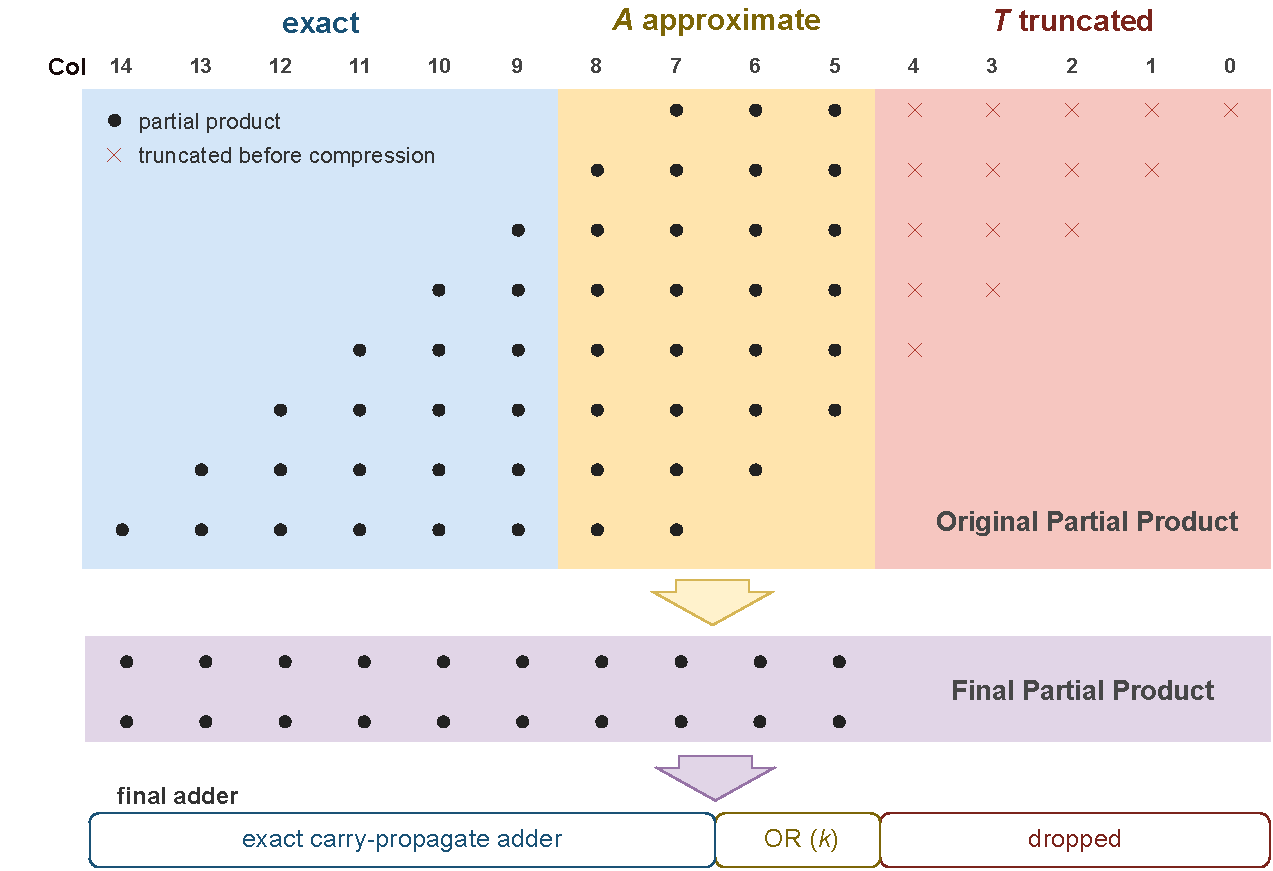
\includegraphics[width=\linewidth]{figs/template}
\Description{Schematic of the parameterised multiplier template: a partial-product array with the T least significant columns removed, a Dadda reduction strip whose (stage, column) slots each carry a compressor-style gene, and a final adder whose k lowest bits are OR-based.}
\caption{The Approx-LG template for $N=8$.  The $T$ truncated columns are
dropped before compression.  Each cell of the reduction strip is one
(stage, column) slot, filled where its compressor style is a gene and hollow
where the template forces an exact adder.  The OR-based $k$ lowest bits belong
to the final adder, not to the tree.}
\label{fig:template}
\end{figure}

The compensation constant is not free.  The mean discarded weight is
$\overline{E}_{T}=\sum_{i<T} w_i 2^{i}$, where $w_i$ sums $1/4$ over the
ordinary partial products of column $i$ and $3/4$ over its inverted ones,
because a Baugh-Wooley array complements the two sign rows; when $T$ exceeds
$N$ the array also loses the correction one at column $N$, of weight $2^{N}$.
The value $c\,\overline{E}_{T}$ folds into the final addition and costs nothing
after constant propagation, so it is a free accuracy knob the search uses
heavily.  Getting it wrong is not a small effect: ignoring the inverted partial
products leaves the signed template with a mean error distance of $2^{15}$ at
$16\times16$, which is why the generator is verified against RTL before any
search runs.

Several genomes decode to the same circuit.  Canonicalisation clips every gene
to its bound, forces $A\le\mathrm{ncol}-T$ and $k\le A$, and zeroes every slot
outside $[T,T+A)$.  A design point is therefore identified by the SHA-1 of its
emitted netlist rather than by its genome, so every algorithm pays for a
circuit exactly once; without that rule an algorithm could buy extra
evaluations by proposing genomes that decode to circuits already seen, and the
budget would stop being a common currency.

\subsection{Iso-flow evaluation}
\label{sec:eval}
\textbf{Accuracy.}  Each wire of the decoded netlist is held as a bit-packed
\texttt{uint64} vector, so one element-wise operation evaluates a gate for 64
input vectors at once.  For $8\times8$ the entire $2^{16}$-point input space
fits in 1024 words per wire and an \emph{exhaustive} characterisation costs
about \MsEight\,ms.  For $16\times16$ the same kernel runs on a GPU over
$2^{22}$ uniformly random operand pairs.  We report \nmed{}, MRE, worst-case
error and error rate.

\textbf{PPA.}  The same genome is emitted as Verilog and pushed through
Yosys~\cite{yosys} (\texttt{synth -flatten}) and ABC~\cite{abc} with
delay-driven mapping and area recovery onto the 45\,nm Nangate Open Cell
Library~\cite{nangate}.  Area comes from \texttt{stat -liberty} and the
critical-path delay from ABC's \texttt{stime}.  Power is obtained by simulating
the \emph{mapped} netlist with the Liberty Boolean functions over $2^{14}$
random operand pairs, measuring the toggle rate $\alpha_n$ of every net and
evaluating
\begin{equation}
P=\tfrac12 V_{dd}^{2} f \sum_{n} C_n\alpha_n + \sum_{c} P^{\mathrm{leak}}_c ,
\end{equation}
with $C_n$ the sum of the Liberty input-pin capacitances of the sinks of net
$n$, $V_{dd}=1.1$\,V and $f=200$\,MHz.  The estimator ignores glitching, so
absolute values are optimistic, but it is applied identically to every design
here.  A failed characterisation is retried and then dropped rather than
cached, since a cached failure would look like a very cheap circuit.  Because
the mapping is delay-driven the absolute numbers are not comparable with
figures published for a commercial flow under a relaxed period constraint, and
our exact $8\times8$ multiplier maps to 541\,$\mu$m$^2$ at 0.54\,ns; every
design here goes through the same recipe, so only within-flow comparisons are
drawn.

\textbf{Verification.}  The three views agree.  For randomly drawn design
points the packed-bit model reproduces Icarus Verilog~\cite{iverilog} over the
complete $2^{16}$-point input space of the $8\times8$ template, unsigned and
signed, and over $4096$ random operand pairs at $16\times16$, in every case
bit-exactly, and it also reproduces the post-ABC mapped netlist.  Of the
\NlibTotal\ published designs collected, \NlibElaborate\ elaborate and expose a
plain integer $N\times N$ interface, and \NlibVerified\ of those also reproduce
their own RTL bit-exactly; only those enter the comparison.  The rest are
floating-point mantissa multipliers, do not elaborate in an open-source
simulator, or leave the product undefined.  Section~\ref{sec:sota16} narrows
\NlibVerified\ further to the \NlibUsed\ that fall inside the error window.

\subsection{LLM guidance}
\label{sec:llm}
\textbf{Symbolic interface.}  A raw genome is a vector of \GenesEight\
integers for $N=8$, which is long, positional and semantically opaque.
Approx-LG instead exchanges a \emph{column-wise record},
\begin{center}\small
\texttt{\{"T":6,"A":4,"comp":2,"cpa\_k":2,\\
"columns":\{"6":"K5","7":"P1","8":["N1",...]\}\}}
\end{center}
which names the style of each approximate column, optionally per stage.  It is
how a designer describes the circuit, an order of magnitude shorter than the
integer vector, and any unknown field is dropped by the decoder.  The prompt
carries the measured $\overline{ED}$ of every style, so the model reasons over
cells it can characterise rather than names it may have memorised.

Fig.~\ref{fig:exchange} shows one complete exchange, verbatim from a campaign
log.  Three properties of the interface matter later.  The model sees a
\emph{summary}, not the population -- the archive in column-wise form plus a
coverage table of how many designs and what best \adp{} each error decade holds
-- which keeps a call inside a couple of thousand tokens however large the
population grows.  The question is about a \emph{position}, the offset $d$
above the truncation point, so one answer applies to every mutation of the
generation and transfers across truncation depths.  And the answer space is
small and closed, a ranked list drawn from the \Nmodes\ styles, so validation
can be total: an answer can be wrong but never malformed in a way the decoder
must guess about.

\begin{figure}[t]
\small
\begin{verbatim}
prompt (tail): NMED in [1e-04,1e-03): 3 designs, best area*delay = 217.2
               NMED in [1e-03,1e-02): 4 designs, best area*delay =  56.0
               Task: for a column d positions above the truncation
               point, list the styles worth trying there, best first.
answer:        {"prior": {"0":  ["A3","A4","OR","K8","N2"],
                          "1":  ["A1","A2","N1","N2","B1"],
                          "2":  ["EXACT","A1","A2","N1","B1"],
                          "3":  ["EXACT","A1","B1","K1","K4"],
                          "4+": ["EXACT","K1","K4","B1","A1"]}}
\end{verbatim}
\Description{A shortened prompt showing a coverage table of Pareto designs per
error decade, followed by the model's JSON answer giving a ranked list of
compressor style names for each column offset from zero to four or more.}
\caption{One elicited proposal distribution, abridged from a campaign log.  The
model never sees or emits a netlist; it ranks named cells for a column
position, and the search samples from that ranking.  This answer shows the
shape every answer has: aggressive cells near the truncation point, the exact
style dominating four or more columns above it.}
\label{fig:exchange}
\end{figure}

\textbf{O1: knowledge-based warm start.}  Half of the initial population is
requested from the model with an instruction to cover four decades of \nmed{}.
The rest comes from the random sampler that seeds every baseline.

\textbf{O2: Pareto-gap candidate injection.}  Every $g_{\mathrm{inj}}=2$
generations the non-dominated archive is shown with a coverage table giving the
population and best \adp{} of each error decade, and $n_{\mathrm{inj}}=6$ new
designs are requested.

\textbf{O3: mutation guidance.}  This operator has two halves, and
Section~\ref{sec:prior} needs them separated.  The first is a \emph{proposal
distribution}: every $g_{\mathrm{pri}}=3$ generations the model ranks the
styles worth trying in a column $d$ positions above the truncation point
($d=0,1,2,3,4^{+}$), returning a short list per offset such as
\texttt{\{"0":["OR","K5"],"1":["A4","K5"],\ldots\}}.  The rank is drawn from a
geometric law with parameter $0.45$ truncated to the list length, and mutation
samples slot genes from it with probability $1-\varepsilon$ and uniformly
otherwise ($\varepsilon=\PriorEps$), so one cheap call biases \emph{every}
mutation of a generation.  The second is a local search: the cheapest design in
each error decade is handed to the model with a request for one dominating
child.

\textbf{O4: search-space refinement.}  Every $g_{\mathrm{ref}}=5$ generations
the model sees the archive and the remaining budget and proposes bounds on $T$,
$A$ and $k$ plus the styles worth keeping.  A restriction is applied by
clipping rather than rejection, so it can never empty the population, the exact
style is always retained, and a truncation range narrower than two columns is
widened so that one generation cannot collapse the front.

\textbf{Fail-closed behaviour.}  Every answer is parsed, range-clipped and
canonicalised, and anything undecodable is discarded and refilled by the
standard operators, so an unusable answer costs latency and not correctness.
The property this buys is weaker than it may look, and we state it carefully.
A run whose endpoint is dead falls back on NSGA-II's \emph{operators}, but it
is not NSGA-II's \emph{run}: the guidance path consumes a different sequence of
random draws, and a well-formed answer that points at an unprofitable region is
not discarded at all, because nothing marks it as wrong.  Fail-closed therefore
bounds the damage in distribution rather than run by run.
Section~\ref{sec:failclosed} measures what is left of it.

\subsection{Controls built into the framework}
\label{sec:controls}
Putting a model inside a search loop creates failure modes that produce
plausible numbers rather than errors, and an experiment that does not defend
against them will report them as results.  Four defences are part of the
framework rather than of the analysis, because each has to act while a run is
in progress.

\textbf{Sham guidance.}  An unguided run is not the right comparison for a
guided one: the guided loop asks for candidates and refills whatever the
operators do not supply, so it consumes a different sequence of random draws
and tops up generations differently.  Any guided configuration can therefore be
run in \emph{sham} mode, in which every operator is invoked, asks its question,
walks its own code path and receives nothing back.  That isolates the model's
content from the control flow carrying it, and Section~\ref{sec:primary} uses
the sham arm as the primary comparison.  The two cannot consume identical random
streams -- an operator returning six candidates and one returning none diverge
by construction -- so this is the closest achievable control, not a perfect
one.

\textbf{Outage detection.}  Because guidance is fail-closed, an endpoint that
stops answering raises no error: the run completes, carries the guided
algorithm's name, and is a run of the unguided one.  Six consecutive failed
calls therefore abort a run, and a completed run whose call-failure rate
exceeds 25\% is discarded rather than written.  We added this after an outage
produced \DeadRuns\ such runs (Section~\ref{sec:failclosed}).

\textbf{Characterisation sanity.}  A synthesis that fails is retried and never
cached, but one returning a number parsed from an incomplete log is
indistinguishable from a good one.  Mapped area rises tightly with the
pre-synthesis cell count, so a design whose area falls below half the
$0.5$th percentile for its own cell count is flagged and re-characterised.
Over \NcharTotal\ characterisations the rule fired \NcharBad\ time: the record
it caught reported \NcharBadArea\ where a fresh synthesis of the same genome
gives \NcharGoodArea, and it had doubled the hypervolume of the run that found
it.

\textbf{Refunding failed characterisations.}  A design whose synthesis cannot
be completed after its retries is dropped and its evaluation refunded to the
budget.  Caching it would be worse than charging it: a failed characterisation
reads as an extremely cheap circuit and would sit on the Pareto front of every
later run that touched it.

\begin{algorithm}[t]
\small
\caption{Approx-LG}
\label{alg:approxlg}
\begin{algorithmic}[1]
\Require budget $B$, population $\mu$, space $\mathcal{G}$
\Ensure non-dominated design set
\State $P\gets\textsc{WarmStart}(\mu/2)\cup\textsc{Random}(\mu/2)$
\State \textsc{Evaluate}$(P)$
\State $\pi\gets\varnothing$, $\rho\gets\varnothing$ \Comment{prior, restriction}
\While{$\mathrm{evals}<B$}
  \State $Q\gets\varnothing$
  \If{$g\bmod g_{\mathrm{inj}}=1$}
     $Q\gets Q\cup\textsc{Inject}(\mathrm{archive},n_{\mathrm{inj}})$
  \EndIf
  \State $Q\gets Q\cup\textsc{GuidedMutate}(\textsc{DecadeElites}(P))$
  \While{$|Q|<\mu$}
     \State $x\gets\textsc{Crossover}(\textsc{Tournament}(P)^2)$
     \State $Q\gets Q\cup\{\textsc{Mutate}(x,\pi,\rho)\}$
  \EndWhile
  \State \textsc{Evaluate}$(Q)$
  \State $P\gets\textsc{EnvSelect}(P\cup Q,\mu)$
  \If{$g\bmod g_{\mathrm{pri}}=1$} $\pi\gets\textsc{ElicitPrior}(\mathrm{archive})$
  \EndIf
  \If{$g\bmod g_{\mathrm{ref}}=0$} $\rho\gets\textsc{Refine}(\mathrm{archive})$
  \EndIf
\EndWhile
\end{algorithmic}
\end{algorithm}

\subsection{The guided loop}
\label{sec:loop}
Algorithm~\ref{alg:approxlg} shows how the four operators plug into an
otherwise textbook NSGA-II.  The initial population that is not warm-started
comes from a sampler shared by every algorithm compared here, which draws
$T=T_{\max}u^{1.7}$ with $u$ uniform, since the error grows as $4^{T}$ and a
uniform draw would put almost every design in the useless high-error corner,
and leaves each slot exact with probability $0.55$.  Parents are picked by
binary tournament on (rank, crowding distance) over the objectives
$(\log_{10}\nmed{},\,\text{area},\,\text{delay})$.  Crossover is uniform on the
four header genes and takes a single column cut through the slot matrix, so a
child inherits a contiguous band of columns from each parent, which keeps
intact the error-cancellation patterns a parent has found.  Mutation perturbs
$T$ and $k$ by $\pm1$ and $A$ by up to $\pm2$ with probabilities $0.25$, $0.20$
and $0.25$, resamples the compensation level with probability $0.15$, and
resamples slot genes at rate $\max(1/L,\,2/|\{m_{s,j}\}|)$ for a genome of
length $L$.

The prior enters at exactly one place.  A resampled slot in column $j$ takes a
uniform style when no prior is available and otherwise draws from
$\pi(\cdot\mid j-T)$, the ranked list for that column offset; conditioning on
$j-T$ rather than $j$ makes the advice transferable across truncation depths.
Because that interface names only an offset and a ranked list, any source can
fill it, which is what Section~\ref{sec:prior} exploits.  Every child is
canonicalised and, when a restriction $\rho$ is active, projected into it.  The
operators are strictly additive: removing all of them leaves plain NSGA-II over
the same template.

The objectives minimised are $(\log_{10}\nmed{},\,\text{area},\,\text{delay})$.
The logarithmic error axis keeps the four useful accuracy decades from
collapsing into a few percent of the objective range and leaves dominance
unchanged, so it buys a crowding distance that spreads the population over
accuracy rather than over the two cheap decades.  Progress is scored by the
hypervolume of the box $\log_{10}\nmed\in[-6,\log_{10}0.02]$,
$\text{area}\in[0,A_{\mathrm{exact}}]$, $\text{delay}\in[0,D_{\mathrm{exact}}]$
normalised to the unit cube, which caps the reward for accuracy no application
needs.  Section~\ref{sec:robust} shows what that cap costs.

The guidance cost is bounded by construction: warm start is one call, and each
generation issues at most one injection, one guided-mutation, one prior and one
refinement call, gated by their periods.  A \Budget-evaluation run at $\mu=32$
issues \LLMcalls\ calls of \LLMsec\,s (\LLMtok\,k tokens): \TimeGuidance\,s
against \TimeEDAcold\,s of synthesis, \GuidanceShare\% of the run.  Guidance is
therefore \emph{not} cheap against an open flow at \SecPerCircuit\,s per
characterisation, only against a commercial one at minutes per synthesis, which
is the regime the budget argument assumes.

\section{Experiments}
\label{sec:exp}
\subsection{Setup}
\label{sec:setup}
All experiments use the flow, objectives and hypervolume box of
Section~\ref{sec:eval} and Section~\ref{sec:loop}.  The \emph{EDA budget} counts
distinct circuits, charged the first time a run asks for one.  All algorithms
use population $\mu=32$, budget $B=400$ ($N=8$) or $B=500$ ($N=16$), and the
same random initialisation; per-arm seed counts are given in each table.  The
LLM endpoint is DeepSeek (\texttt{\LLMname}) with extended thinking disabled.
Experiments ran on a 32-core workstation with an RTX~4060, every tool is open
source and the rest pure Python, so the campaign reproduces without an EDA
licence.  The framework, the campaign drivers, the analysis scripts and the
search traces every figure and table in this paper is computed from are
available for review at
\url{https://anonymous.4open.science/r/Approx-LG-71AA/}.

\textbf{Cost.}  Wall-clock time is reported per component, not per run, because
the persistent characterisation cache makes a run's measured time depend on
what earlier campaigns happened to have synthesised.  Pooled over every timed
run one characterisation costs \SecPerCircuit\,s, so a \Budget-evaluation run
spends about \TimeEDAcold\,s in the EDA flow whichever algorithm asks; guidance
adds \TimeGuidance\,s on top of that (Section~\ref{sec:loop}).

\textbf{Which runs count.}  Failed calls are refilled by the standard
operators, so a run whose calls all failed still completes and is still
labelled Approx-LG, and averaging such runs into the guided arm dilutes the
effect towards zero.  Runs with a call-failure rate above 25\% are discarded;
Section~\ref{sec:failclosed} reports what happened when we had \DeadRuns\ of them.

\subsection{Statistical protocol}
\label{sec:stats}
This paper compares many arms under many scorings, and the number of tests is
large enough that reporting a $p$-value per comparison would be misleading on
its own.  We therefore fix the protocol before the results.

\textbf{Primary endpoint.}  One comparison carries the paper's claim: the
guided arm against the \emph{sham} arm of Section~\ref{sec:controls}, at each
width.  Everything else -- the reference baselines, the prior sources, the
ablation, the reference boxes -- is secondary, and each of those families is
corrected within itself by Holm's step-down procedure, which assumes nothing
about the dependence between the tests it corrects.
Section~\ref{sec:primary} reports that one comparison, ahead of every secondary
family.

\textbf{Pairing and the test.}  A seed also seeds the initial population, which
the same sampler draws for every arm, so runs pair by seed and the paired test
is the powerful one.  Wilcoxon's signed-rank statistic is computed
\emph{exactly} for $n\le24$ by enumerating the $2^n$ sign assignments rather
than through the normal approximation.  This matters at the seed counts here:
at $n=8$ the two-sided $p$ lives on a grid whose smallest value is $1/128
\approx 0.008$, and an approximation that returns $0.03$ at that sample size is
reporting a number the test cannot produce.

\textbf{Effect sizes.}  Every comparison carries a paired mean relative
difference with a percentile bootstrap interval over $20{,}000$ resamples and
$\hat{A}_{12}$, the probability that a run of one arm beats a run of the other.
An interval says more than a threshold, because it also bounds how large the
effect could plausibly be.

\textbf{What the pipeline invents from nothing.}  A significance threshold does
not say whether an effect is larger than the noise this particular pipeline
generates, so we measure that directly: one arm's runs are split into two
disjoint halves at random and scored against each other exactly as a real
comparison would be, two thousand times.  For NSGA-II at $8\times8$ the
absolute difference so produced has a median of \NullEightMed\% and a 95th
percentile of \NullEightN\%; for the guided arm, whose runs are more variable,
the 95th percentile is \NullEight\%.  At $16\times16$ it is \NullSixteen\%.
Any effect inside that band is not evidence, whatever its $p$-value, and we
say so where it applies rather than leaning on the threshold.

\subsection{The primary comparison}
\label{sec:primary}
Every other arm in this section differs from the guided one in more than the
model's content.  The endpoint fixed in Section~\ref{sec:stats} does not: the
guided arm and the sham arm of Section~\ref{sec:controls} walk the same control
flow, ask the same questions at the same points and differ only in whether the
answers are used, so what separates them is what the answers \emph{say}.  The
two arms share \ShamSixteenUN\ seeds at each width and pair by seed.  On the
$16\times16$ unsigned template guidance is worth \ShamSixteenU\% of final
hypervolume (95\% bootstrap CI \ShamSixteenUCI), winning \ShamSixteenUWins\
pairs at an exact Wilcoxon $p\le\ShamSixteenUP$, which Holm's correction within
the primary family leaves at $\le\ShamSixteenUHolm$, and
$\hat{A}_{12}=\ShamSixteenUA$.  On the signed template it is \ShamSixteenS\%
(CI \ShamSixteenSCI, \ShamSixteenSWins\ pairs, $p\le\ShamSixteenSHolm$
corrected, $\hat{A}_{12}=\ShamSixteenSA$).  At $8\times8$ the point estimate is
just as large, \ShamEight\% (CI \ShamEightCI, \ShamEightWins\ pairs), but the
interval covers zero and the test does not reject: $p=\ShamEightP$, which the
correction leaves at $p=\ShamEightHolm$, with $\hat{A}_{12}=\ShamEightA$.

The $8\times8$ number is not a small effect measured precisely, and the null
band of Section~\ref{sec:stats} disposes of it without appeal to any threshold:
scoring one arm's runs against a random split of themselves produces absolute
differences with a median of \NullEightMed\% and a 95th percentile of
\NullEight\% for the guided arm (\NullEightN\% for NSGA-II), so a difference of
\ShamEight\% is inside the range this pipeline manufactures from nothing.  We
therefore do not claim it, at either sign of the effect.  At $16\times16$ the
band is \NullSixteen\%: the unsigned interval lies above it entirely, while the
signed effect clears it as a point estimate with an interval that still reaches
into it.  The claim the paper carries is accordingly the narrow one.  On the
larger template, where $500$ evaluations leave the space far from exhausted,
the content of the model's answers -- not the loop that fetches them -- is worth
a real and repeatable gain in hypervolume; at $8\times8$, where the space is
small enough that the standard operators find the same front on their own, we
have no evidence that it is worth anything.  Everything from
Section~\ref{sec:ablation} onwards is secondary by construction, and is read as
description rather than as confirmation.

\subsection{Search efficiency and ablation}
\label{sec:ablation}
\begin{figure}[t]
\centering
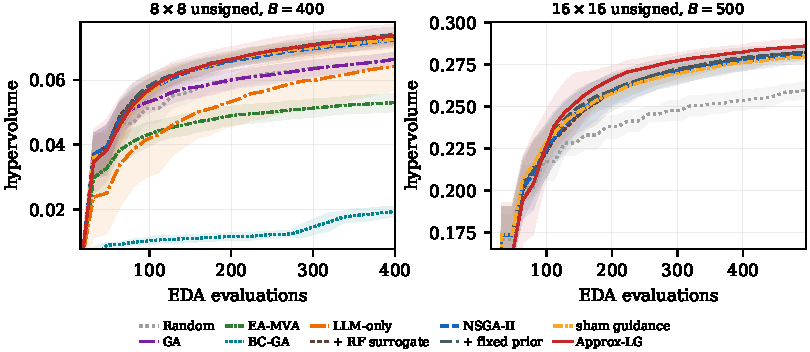
\includegraphics[width=\linewidth]{figs/hv_both}
\Description{Two line plots of hypervolume against the number of EDA evaluations, one for the 8x8 template and one for the 16x16 unsigned template, with one curve per search algorithm and a shaded one-sigma band around each.}
\caption{Hypervolume against EDA budget (mean, shaded $\pm1\sigma$), $8\times8$
and $16\times16$ unsigned; per-arm run counts are in Tables~\ref{tab:search}
and~\ref{tab:prior}.  ``$+$ fixed prior'' and ``$+$ RF surrogate'' are NSGA-II
with the written designer prior of Section~\ref{sec:prior} and with the
surrogate-assisted loop of Section~\ref{sec:surrogate}.  ``Sham guidance'' is
the placebo of Section~\ref{sec:controls}: the guided control flow with every
answer discarded, and it, not NSGA-II, is the curve Approx-LG has to beat.
Axes start at the second generation.}
\label{fig:hv}
\end{figure}

\begin{table}[t]
\caption{Search performance on $8\times8$ multipliers ($B=400$).}
\label{tab:search}
\centering\footnotesize
\setlength{\tabcolsep}{3pt}
\begin{tabular}{lccccc}
\toprule
method & runs & hypervolume & $|PF|$ & evals.\ to & time\\
       &      &             &        & NSGA-II HV & (s)\\
\midrule
% generated by scripts/analyze_search.py
Random & 30 & 0.0664 $\pm$ 0.0022$^{\dagger}$ & 80 & 400~(0/30) & 39 \\
GA & 30 & 0.0664 $\pm$ 0.0022$^{\dagger}$ & 82 & 400~(0/30) & 102 \\
NSGA-II & 30 & 0.0724 $\pm$ 0.0018 & 115 & 375~(15/30) & 86 \\
EA-MVA~\cite{devi2025} & 30 & 0.0530 $\pm$ 0.0028$^{\dagger}$ & 90 & 400~(0/30) & 52 \\
BC-GA~\cite{wen2025} & 30 & 0.0194 $\pm$ 0.0017$^{\dagger}$ & 62 & 400~(0/30) & 56 \\
LLM-only & 30 & 0.0642 $\pm$ 0.0077$^{\dagger}$ & 90 & 383~(5/30) & 345 \\
NSGA-II\,+\,fixed prior & 20 & 0.0741 $\pm$ 0.0023 & 116 & 332~(15/20) & 118 \\
NSGA-II\,+\,elicited prior & 20 & 0.0723 $\pm$ 0.0019 & 118 & 364~(9/20) & 174 \\
NSGA-II\,+\,RF surrogate & 30 & 0.0729 $\pm$ 0.0017 & 120 & 361~(19/30) & 198 \\
sham guidance & 20 & 0.0726 $\pm$ 0.0022 & 113 & 358~(12/20) & 99 \\
Approx-LG & 30 & 0.0737 $\pm$ 0.0036 & 122 & 338~(20/30) & 263 \\

\bottomrule
\end{tabular}

\smallskip
{\footnotesize $^{\dagger}$~difference to Approx-LG significant at $p<0.05$
(Mann--Whitney~U).  Seed counts differ by arm because the prior controls of
Section~\ref{sec:prior} were added later, at \SeedsExpert\ seeds each.}
\end{table}

Figure~\ref{fig:hv} and Table~\ref{tab:search} give the budget-matched
comparison.  Approx-LG's mean curve stays above NSGA-II's from \LeadFrom\
evaluations to the end of the budget, and its final hypervolume is
\HVgainEight\% higher over \SeedsEight\ runs (Mann--Whitney $p=\UnpairedP$,
$\hat{A}_{12}=\EffectA$).  The seed also seeds the initial population, drawn by
the same sampler for every algorithm, so runs pair up and the paired test is
the more powerful one: Approx-LG wins \PairedWins\ of the pairs against NSGA-II
by \PairedGain\% on average (Wilcoxon $p=\PairedP$), and essentially every pair
against random search, the GA, the two reproduced methods and the LLM-only
searcher ($p\le0.03$ each).  \emph{Against NSGA-II itself the difference is not
significant}, and we say so rather than lean on the \SeedsEight-seed mean: an
effect this size needs many more runs or a larger problem, and
Section~\ref{sec:hv16} supplies the second.  The first ten seeds of this campaign
gave $\PairedGainTen$\%, well above where the full set settles.  The mean
trajectory reaches the hypervolume NSGA-II attains with the \emph{full} budget
after \EvalsApproxLG\ evaluations, a \SpeedupEight$\times$ reduction in EDA
effort.  The two reproduced methods sit lowest because each explores only a
sub-space of the template: \cite{devi2025} has neither compensation nor an
approximate final adder and \cite{wen2025} never truncates.  That is not a
defect of the reproduction, whose designs reach the area reductions its authors
report, but a compressor-only method cannot enter the cheap corner the
hypervolume rewards.

The LLM-only searcher is instructive: competitive over the first hundred
evaluations, because circuit knowledge alone starts it quickly, but with no
mechanism for local refinement it ends \emph{below} plain NSGA-II, so asking a
model to run the whole search is markedly worse than using it to steer one.
Across all runs \LLMfrontShare\% of the final Pareto points came from an LLM
operator.

\begin{table}[t]
\caption{Contribution of each guidance operator ($8\times8$, $B=400$).
$\Delta$ and $p$ are paired against the full system on the seeds the two
share.  The last row is plain NSGA-II, that is, every operator removed at
once.}
\label{tab:ablation}
\centering\small
\setlength{\tabcolsep}{5pt}
\begin{tabular}{lcccc}
\toprule
variant & runs & hypervolume & $\Delta$ & $p$\\
\midrule
Approx-LG & 30 & 0.0737 $\pm$ 0.0036 & -- & -- \\
w/o warm start & 20 & 0.0739 $\pm$ 0.0026 & -0.1\% & 1.00 \\
w/o candidate injection & 20 & 0.0727 $\pm$ 0.0018 & -1.8\% & 0.18 \\
w/o mutation guidance & 20 & 0.0722 $\pm$ 0.0020 & -2.4\% & 0.18 \\
w/o the proposal distribution & 20 & 0.0743 $\pm$ 0.0030 & +0.4\% & 1.00 \\
w/o space refinement & 20 & 0.0727 $\pm$ 0.0028 & -1.7\% & 0.35 \\
no guidance ($=$ NSGA-II) & 30 & 0.0724 $\pm$ 0.0018 & -1.6\% & 0.25 \\

\bottomrule
\end{tabular}
\end{table}

Table~\ref{tab:ablation} removes one operator at a time.  \AblationText

\subsection{Does the guidance need a language model?}
\label{sec:prior}

\begin{table}[t]
\caption{Where the ranked style lists come from ($8\times8$, $B=400$).  Every
arm is the same NSGA-II and differs only in the provenance of the proposal
distribution.  $\Delta$, wins and $p$ are paired against uniform sampling on
the same seeds.}
\label{tab:prior}
\centering\footnotesize
\setlength{\tabcolsep}{3pt}
\begin{tabular}{lccccc}
\toprule
proposal distribution & runs & hypervolume & $\Delta$ & wins & $p$\\
\midrule
% generated by scripts/analyze_priors.py
uniform (NSGA-II) & 30 & 0.0724 $\pm$ 0.0018 & -- & -- & -- \\
fixed designer prior & 20 & 0.0741 $\pm$ 0.0023 & +2.6\% & 16/20 & $<$0.01 \\
adaptive prior (UCB) & 20 & 0.0720 $\pm$ 0.0018 & -0.2\% & 11/20 & 0.74 \\
elicited prior (LLM) & 20 & 0.0723 $\pm$ 0.0019 & +0.3\% & 10/20 & 0.88 \\
Approx-LG (all four operators) & 30 & 0.0737 $\pm$ 0.0036 & +1.9\% & 17/30 & 0.25 \\

\bottomrule
\end{tabular}
\end{table}

An ablation that deletes an operator cannot say whether the \emph{model} or the
\emph{channel} matters.  Table~\ref{tab:prior} asks directly, with arms sharing
everything but provenance: sampler, crossover, mutation rates, $\varepsilon$,
the geometric rank draw and the refresh period are identical, and only the
source of $\pi(\cdot\mid j-T)$ changes.  The \emph{fixed} prior is written from
the rule of Section~\ref{sec:space} and never fitted: the error a cell may
contribute halves per column above the truncation point, so styles are ranked
by the distance of their measured $\overline{|ED|}$ from $\tau_{\max}2^{-d}$
and the list is reordered to alternate bias sign.  The \emph{adaptive} prior
re-estimates the same lists every $g_{\mathrm{pri}}$ generations from how much
more often a style appears at an offset among the non-dominated designs than
among everything evaluated, with a UCB term, so it sees strictly more about the
run in progress than the model does.

The two are not the same advice.  Over \NPriorAnswers\ elicited answers at
$8\times8$ the head of the model's list matches the fixed one for
\PriorHeadMatch\% of offsets and lies in its top three for \PriorTopThree\%.
They agree on \emph{shape}, both making the tolerable cell error fall with the
offset and both putting the exact style first five columns up (the model in
\PriorExactFar\% of answers), and disagree at the truncation boundary, where
the rule names the library's most aggressive cell and the model a milder one.
\PriorText

\subsection{The other way to spend a small budget}
\label{sec:surrogate}
Injecting knowledge from outside is not the standard answer to an expensive
evaluation; learning a cheap model of it is, and a surrogate-assisted loop
competes for exactly the same resource.  Ours is a textbook one: every truly
evaluated point trains a random forest per objective, the standard operators
produce a pool sixteen times the population, the forests rank it, and only the
predicted front reaches the EDA flow, with $15\%$ of each generation filled at
random so a confident but wrong surrogate cannot lock the search in.  It gets
the same circuit knowledge the priors reason over -- the measured error
statistics of the assigned cells -- not raw style indices.

At $8\times8$ it lands between NSGA-II and Approx-LG with nothing separating
the three.  \SurrogateText\ It is a real method rather than a straw man,
recovering roughly half of what guidance buys, and the guided arm beats it on
one template of two.

\subsection{\texorpdfstring{Scaling to $16\times16$}{Scaling to 16x16}}
\label{sec:hv16}

\begin{table}[t]
\caption{Search performance at $16\times16$ ($B=500$), unsigned above and
signed below.  Columns are those of Table~\ref{tab:search}.  These are the arms
the primary comparison of Section~\ref{sec:primary} pairs by seed.}
\label{tab:search16}
\centering\footnotesize
\setlength{\tabcolsep}{3pt}
\begin{tabular}{lccccc}
\toprule
method & runs & hypervolume & $|PF|$ & evals.\ to & time\\
       &      &             &        & NSGA-II HV & (s)\\
\midrule
\multicolumn{6}{l}{\emph{unsigned}}\\
% generated by scripts/analyze_search.py
Random & 8 & 0.2600 $\pm$ 0.0054$^{\dagger}$ & 79 & 500~(0/8) & 113 \\
NSGA-II & 20 & 0.2811 $\pm$ 0.0046$^{\dagger}$ & 126 & 458~(12/20) & 153 \\
NSGA-II\,+\,fixed prior & 20 & 0.2826 $\pm$ 0.0027$^{\dagger}$ & 133 & 437~(15/20) & 144 \\
sham guidance & 20 & 0.2798 $\pm$ 0.0029$^{\dagger}$ & 127 & 472~(7/20) & 137 \\
Approx-LG & 20 & 0.2863 $\pm$ 0.0046 & 132 & 374~(18/20) & 322 \\

\midrule
\multicolumn{6}{l}{\emph{signed}}\\
% generated by scripts/analyze_search.py
Random & 8 & 0.1792 $\pm$ 0.0060$^{\dagger}$ & 72 & 500~(0/8) & 116 \\
NSGA-II & 20 & 0.1990 $\pm$ 0.0049$^{\dagger}$ & 115 & 436~(14/20) & 128 \\
NSGA-II\,+\,fixed prior & 20 & 0.2018 $\pm$ 0.0022$^{\dagger}$ & 120 & 420~(19/20) & 103 \\
sham guidance & 20 & 0.2009 $\pm$ 0.0034$^{\dagger}$ & 114 & 423~(14/20) & 114 \\
Approx-LG & 20 & 0.2042 $\pm$ 0.0028 & 118 & 321~(20/20) & 338 \\

\bottomrule
\end{tabular}

\smallskip
{\footnotesize $^{\dagger}$~difference to Approx-LG significant at $p<0.05$
(Mann--Whitney~U).  Random search is run at fewer seeds because it is not a
contender for the endpoint.}
\end{table}

At $16\times16$ the genome has \GenesSixteen\ entries instead of \GenesEight,
$500$ evaluations are far from saturating the space, and the template is a
different one, signed in half the runs.  This is the transfer test the
$8\times8$ result asks for: the rule was stated once in general terms and is
applied here unchanged, while the model is asked the same question about a
different circuit.  Table~\ref{tab:search16} gives both templates arm by arm,
including the sham arm that Section~\ref{sec:primary} pairs against.
\SixteenText

\subsection{The budget the paper counts, and the one a user pays}
\label{sec:walltime}
Counting EDA evaluations is the right currency only when an evaluation
dominates the run.  On this flow it does not.  A characterisation costs
\SecPerCircuitWide\,s and guidance costs \GuidanceSecondsWide\,s, so an
evaluation budget quietly hands the guided arm minutes that the unguided arms
could have spent evaluating.  We therefore re-ran NSGA-II, the sham arm and the
surrogate at the budget those minutes actually buy, \EqTimeEvals\ evaluations
instead of $500$, and compared every arm at the wall clock the guided run
reaches its own budget at, \EqTimeSeconds\,s.

\emph{Under that accounting the guided arm loses.}  It is \EqTimeNSGA\%
against NSGA-II (CI \EqTimeNSGACI, $p=\EqTimeNSGAP$), \EqTimeRF\% against the
surrogate ($p=\EqTimeRFP$) and \EqTimeSham\% against the sham arm
($p=\EqTimeShamP$).  The \ShamSixteenU\% it gains per evaluation is smaller
than what the same seconds buy in extra evaluations.

This does not overturn the evaluation-budget result; it prices it.  NSGA-II
needs a median of \MatchNSGA\ evaluations to reach the guided arm's final
hypervolume, and \GuidanceSecondsWide\,s of guidance is worth that difference
only once a characterisation costs \BreakEvenNSGA\,s; against the surrogate the
threshold is \BreakEvenRF\,s and against the sham arm \BreakEvenSham\,s.  Our
open flow sits at \SecPerCircuitWide\,s, a factor of three below the cheapest
of those, which is why guidance loses here.  A commercial flow at minutes per
synthesis sits two orders of magnitude above them.  The honest statement is
therefore conditional, and the condition is measurable: \emph{guidance of this
cost is worth buying when one characterisation costs more than about a second},
and every number in this paper was produced in a regime where it does not.

\subsection{Robustness of the comparison}
\label{sec:robust}

\begin{table}[t]
\caption{The $8\times8$ comparison re-scored under other reference boxes and
under two indicators that use none.  $\Delta$, wins and $p$ are Approx-LG
against NSGA-II, paired by seed; a positive $\Delta$ always favours
Approx-LG.}
\label{tab:hvsens}
\centering\footnotesize
\setlength{\tabcolsep}{3pt}
\begin{tabular}{lccccc}
\toprule
scoring & NSGA-II & Approx-LG & $\Delta$ & wins & $p$\\
\midrule
% generated by scripts/analyze_robustness.py
default ($\eta\in[10^{-6},0.02]$, log) & 0.0724 & 0.0737 & +1.9\% & 17/30 & 0.25 \\
tight cap ($\eta\le 0.005$) & 0.0316 & 0.0320 & +1.3\% & 14/30 & 0.81 \\
loose cap ($\eta\le 0.05$) & 0.1160 & 0.1198 & +3.3\% & 26/30 & $<$0.01 \\
deep floor ($\eta\ge 10^{-7}$) & 0.0588 & 0.0598 & +1.9\% & 17/30 & 0.25 \\
shallow floor ($\eta\ge 10^{-5}$) & 0.0925 & 0.0943 & +2.1\% & 19/30 & 0.14 \\
linear error axis & 0.2931 & 0.2988 & +2.0\% & 24/30 & 0.01 \\
relaxed cost reference ($1.2\times$) & 0.1411 & 0.1416 & +0.4\% & 16/30 & 0.75 \\
$I_{\varepsilon+}$ (lower better) & 0.0898 & 0.0996 & -12.0\% & 18/30 & 0.97 \\
IGD$+$ (lower better) & 0.0107 & 0.0163 & -51.6\% & 14/30 & 0.20 \\

\bottomrule
\end{tabular}
\end{table}

\RobustText

\subsection{What a guidance outage costs}
\label{sec:failclosed}
\FailClosedText

\subsection{Evolutionary baselines}
\label{sec:evoref}
Both reference methods were re-implemented inside our template from the cell
definitions and algorithm descriptions of the papers and run at the same
budget.  Pooling the non-dominated designs of all \SeedsEight\ runs of each
gives \NrefEight\ reference points -- ours, not published ones -- and for each
we take the Approx-LG design at least as accurate: Approx-LG has a lower
\adp{} in \SotaEightADP\% of those comparisons and a lower \pdp{} in
\SotaEightPDP\%, median \adp{} reduction \MedianADPEight\%.  The improvement
comes from two things neither method has, joint optimisation of truncation
\emph{and} compressor styles, and the compensation constant with the OR-based
final adder.

\subsection{Published libraries}
\label{sec:sota16}

\begin{figure}[t]
\centering
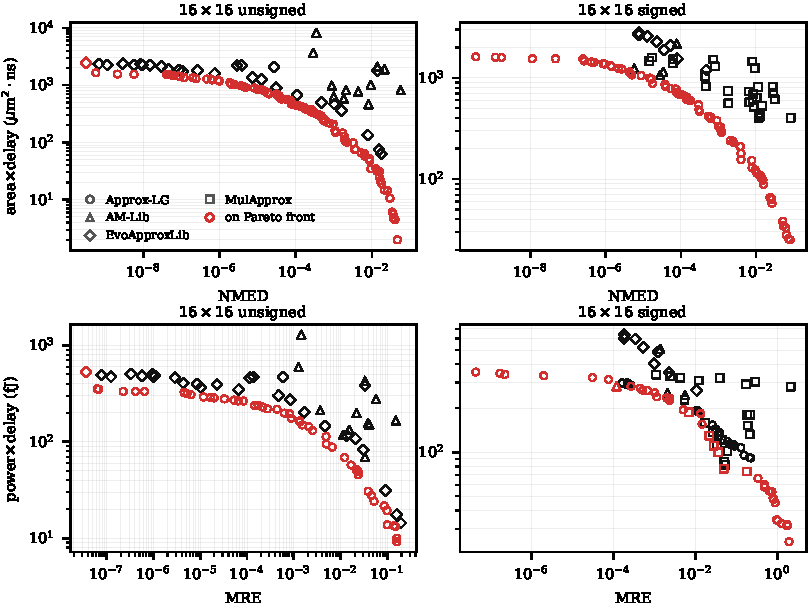
\includegraphics[width=\linewidth]{figs/sota16}
\Description{Four scatter plots of published and generated 16x16 multipliers, unsigned and signed templates in columns and the area-delay and power-delay planes in rows, with error on the horizontal axis and cost on the vertical axis.}
\caption{Approx-LG against \NrefSixteen\ published $16\times16$ designs of
AM-Lib~\cite{amlib}, MulApprox~\cite{mulapprox} and
EvoApproxLib~\cite{evoapproxlib,mrazek2017,mrazek2020} through the same recipe.
Columns are the two templates, rows the two cost planes; shape gives a design's
origin, and a marker is red when it lies on the Pareto front of
\emph{everything} in its panel.  Each panel is clipped to the error range its
published designs occupy: the search also returns points beyond it, with
relative errors above 100\%, and drawing them stretches both axes by two
decades around a region no application uses.  Nothing is excluded from the
rates, only from the picture, and a design outside that range has no reference
to be compared against in any case.  The rates in the text are stricter than
the panels, requiring \nmed{} \emph{and} MRE together.}
\label{fig:sota16}
\end{figure}

The strongest test uses designs we did not produce.  We synthesised every
combinational $16\times16$ multiplier of AM-Lib~\cite{amlib},
MulApprox~\cite{mulapprox} and EvoApproxLib~\cite{evoapproxlib} with the
identical recipe and simulator; the last is the natural yardstick, being the
reference library of the field and itself the product of gate-level
evolution~\cite{vasicek2015,mrazek2017,mrazek2020}.  The counts are:
\NlibTotal\ designs collected, \NlibElaborate\ that elaborate and expose a
plain integer $16\times16$ interface, \NlibVerified\ of those reproducing their
own RTL bit-exactly, and \NlibUsed\ inside the error window the comparison
covers.  The \NlibExcluded\ dropped above it show an \nmed{} beyond 10\,\% in
the input convention we could reconstruct and are excluded rather than counted
as easy wins; the \NlibExact\ dropped below it are exact multipliers, two Booth
designs from AM-Lib and two from EvoApproxLib.  A reference counts as beaten
only if some Approx-LG
design is at least as good on \emph{both} \nmed{} and MRE and is strictly
cheaper.  This section compares \emph{frameworks}, not guidance: the fronts are
the union of the guided runs, and the template, the compensation constant and
the iso-flow evaluation do the larger part of the work.

Figure~\ref{fig:sota16} places the front against all \NrefSixteen\ references in
both cost planes.  The second row is the harder test, because MRE punishes
exactly what truncation buys, yet the front stays below the published designs
there too.  Approx-LG improves the area--delay product of \SotaSixteenADP\% of
the references and the power--delay product of \SotaSixteenPDP\%, with a median
reduction of \MedianADPSixteen\% (\MedianPDPSixteen\% for \pdp{}); per library
the rate is \SotaAm\% over \NrefAm\ AM-Lib designs, \SotaEvo\% over \NrefEvo\
EvoApproxLib designs and \SotaMul\% over \NrefMul\ MulApprox designs.  The
EvoApproxLib figure is the informative one, because those circuits come from
gate-level evolution with a far larger budget over the same accuracy range, so
beating \SotaEvo\% of them suggests template plus circuit knowledge is worth
more than unrestricted gate-level freedom at this budget.  The losses are
instructive too: almost all are \emph{logarithmic} multipliers in the $10^{-3}$
to $10^{-2}$ band, where the log domain is a structural advantage a
Baugh-Wooley array cannot imitate, and the rest sit below
$\nmed{}=10^{-7}$, where the hypervolume box stops rewarding accuracy, the same
blind spot Section~\ref{sec:robust} finds with IGD$+$.



\subsection{Learned structure and applications}

\begin{table}[t]
\caption{Application quality along the Approx-LG $8\times8$ front.  Each design
is followed by the published design of matching \nmed{}.  ``Lossless'' means
every one of the six images came back bit-exact, so the PSNR is infinite rather
than large.}
\label{tab:apps}
\centering\scriptsize
\setlength{\tabcolsep}{2.2pt}
\begin{tabular}{lccccccc}
\toprule
\multirow{2}{*}{design} & \multirow{2}{*}{\nmed{}} & \multirow{2}{*}{MRE} &
\pdp{} & \multicolumn{2}{c}{PSNR (dB)} & SSIM & LeNet-5\\
\cmidrule(lr){5-6}
 & & & (fJ) & blend & smooth & (blend) & top-1\\
\midrule
exact & 0 & 0 & 66.6 & -- & -- & 1.0000 & 98.18\% \\
ALG-1 & 1.92e-06 & 0.0001 & 53.3 & lossless & 63.7 & 1.0000 & 98.15\% \\
mul8u\_Y48 & 1.92e-06 & 0.0001 & 78.1 & lossless & 63.7 & 1.0000 & 98.15\% \\
ALG-2 & 1.08e-05 & 0.0003 & 51.7 & lossless & 60.7 & 1.0000 & 98.16\% \\
mul8u\_125K & 9.61e-06 & 0.0002 & 77.8 & 61.3 & 60.5 & 0.9997 & 98.18\% \\
ALG-3 & 1.18e-04 & 0.0032 & 46.4 & 56.5 & 50.3 & 0.9992 & 98.17\% \\
mul8u\_QJD & 1.73e-04 & 0.0051 & 75.8 & 56.2 & 50.2 & 0.9992 & 98.25\% \\
ALG-4 & 6.29e-04 & 0.0121 & 39.8 & 51.3 & 38.8 & 0.9983 & 98.31\% \\
mul8u\_NGR & 6.50e-04 & 0.0190 & 56.9 & 54.2 & 40.3 & 0.9987 & 98.26\% \\
ALG-5 & 2.46e-03 & 0.1056 & 23.4 & 48.7 & 29.1 & 0.9970 & 97.23\% \\
mul8u\_DM1 & 2.06e-03 & 0.0473 & 50.7 & 48.1 & 30.2 & 0.9966 & 98.25\% \\
ALG-6 & 8.62e-03 & 0.4520 & 10.2 & 39.5 & 13.8 & 0.9775 & 60.77\% \\
ALM\_SOA\_W12 & 8.41e-03 & 0.0343 & 99.7 & 35.9 & 41.6 & 0.9661 & 98.16\% \\

\bottomrule
\end{tabular}
\end{table}

The search does not converge on a single best compressor.
6 styles cover 77.3\,\% of the approximate slots, and they mix under-estimating cells (\texttt{A4}, \texttt{K5}, \texttt{OR} at $\overline{ED}=+0.38,\,+0.75,\,+0.62$, 34.6\,\%) with over-estimating ones (\texttt{A3}, \texttt{N2} at $\overline{ED}=-0.38$, 22.8\,\%) and the balanced \texttt{B1} (19.8\,\%), the error-cancellation mechanism that motivates
biased compressors~\cite{wen2025} ($\overline{ED}$ is the mean error distance
of a style's 3:2 cell, positive when it under-estimates).  Aggressive OR-style
cells sit just above the truncation point and five columns higher the
population reverts to balanced or exact cells, the structure both priors
describe.

Table~\ref{tab:apps} evaluates a slice of the front on three workloads: image
blending and $5\times5$ Gaussian smoothing over six standard images, and
LeNet-5 on MNIST with every multiplication replaced by the approximate one
(8-bit quantisation, exact accumulation, a $256\times256$ product table from
the synthesised model).  \AppsText

\begin{figure}[t]
\centering
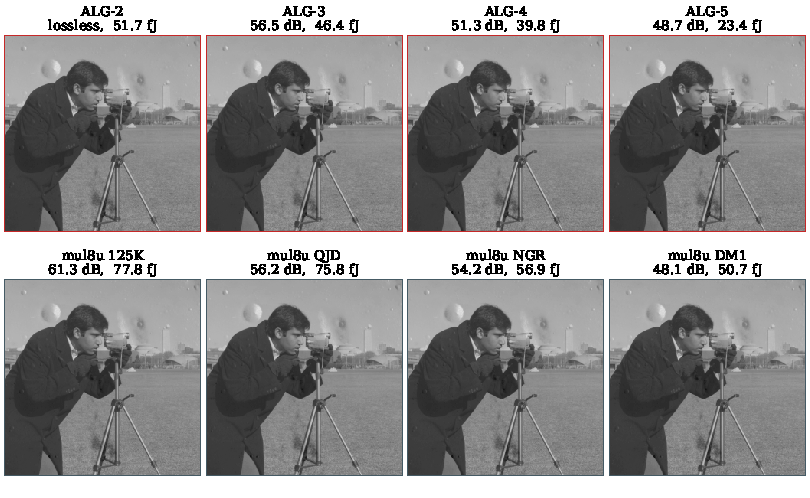
\includegraphics[width=\linewidth]{figs/apps_blend}
\Description{Eight greyscale photographs of a cameraman blended with a picture
of the moon, arranged in four columns and two rows.  The top row is produced by
four Approx-LG designs and the bottom row by the published design of matching
accuracy in each column.  The images in a column look the same as each other.}
\caption{Image blending through four iso-accuracy pairs.  Each column is one
pair: an Approx-LG design (top, red border) above the published design of
matching \nmed{} (bottom); accuracy decreases left to right.  Panel labels give
the PSNR against the exact multiplier and the power--delay product, both taken
from Table~\ref{tab:apps}, so the figure and the table cannot drift; the PSNR
averages the six standard images while one of them is shown.  The claim the
figure makes is the energy one, and it holds in every column: the Approx-LG
design costs 30 to 54\% less while the two images are indistinguishable.  It
makes no claim about which side wins on PSNR, because at matched accuracy that
is noise -- ours is ahead in three of these four blends and, over both
workloads of Table~\ref{tab:apps}, in five of the eight pairs.}
\label{fig:appsblend}
\end{figure}


Fig.~\ref{fig:appsblend} shows what those numbers look like on the blend.
Reading down a column rather than across a row is the point: the two designs in
a column are matched on \nmed{} and MRE, they are matched on the page too, and
the Approx-LG design of the pair is the cheaper one in every column.  That is
the whole of the application claim.  It is worth saying what the figure does
\emph{not} show: at matched accuracy the PSNRs are within a decibel or two
either way -- across both workloads ours is higher in five of the eight pairs
and lower in three -- and we do not read anything into that split.  Reading
across a row shows how the front degrades, and smoothing degrades faster than
the blend because each output pixel accumulates twenty-five products instead of
two, which is why its PSNR column in Table~\ref{tab:apps} falls away first.

\section{Conclusion}
A language model is useful in approximate-circuit design not as an RTL writer
but as a \emph{search operator}, and the controls say which kind.  A proposal
distribution over compressor styles, conditioned on the column offset, is a
real mechanism: filled from a written rule it is the single largest improvement
to NSGA-II we measured, and filled from the run's own data it does nothing, so
the knowledge must come from outside the search.  But the model is not the
better source for it at any width, and the guided system keeps most of its
advantage with that channel removed.  What the model supplies is \emph{candidate
designs} -- a warm start, injections into Pareto gaps, a child asked to
dominate a decade elite -- not a policy for the mutation operator, which is
close to the opposite of what we set out to show.  \SixteenVerdict.

The size of what it supplies should be stated as plainly as its nature.
Against the placebo it is worth a couple of percent of hypervolume at
$16\times16$ and nothing resolvable at $8\times8$; a surrogate model recovers
about half of it with no inference at all; and under a wall-clock budget on an
open flow it is negative, turning positive only where a characterisation costs
about \BreakEvenNSGA\,s or more.  Every candidate stays correct by construction
and the fronts beat \SotaSixteenADP\% of \NrefSixteen\ published designs at
equal \nmed{} \emph{and} MRE -- though an arm with no model in it reaches
\SotaShamSixteenADP\% of the same library, which is where the credit for that
number mostly belongs.
We would urge anyone reporting LLM-guided optimisation to run the placebo and
the fixed-prior control before concluding that the model is what helped.

\bibliographystyle{ACM-Reference-Format}
\bibliography{refs}

\end{document}
